%\documentclass[convert]{standalone}
\documentclass[tikz,border=2pt]{standalone}
\usepackage{mhchem}
\usepackage{chemfig}
\usepackage{siunitx}
\begin{document}
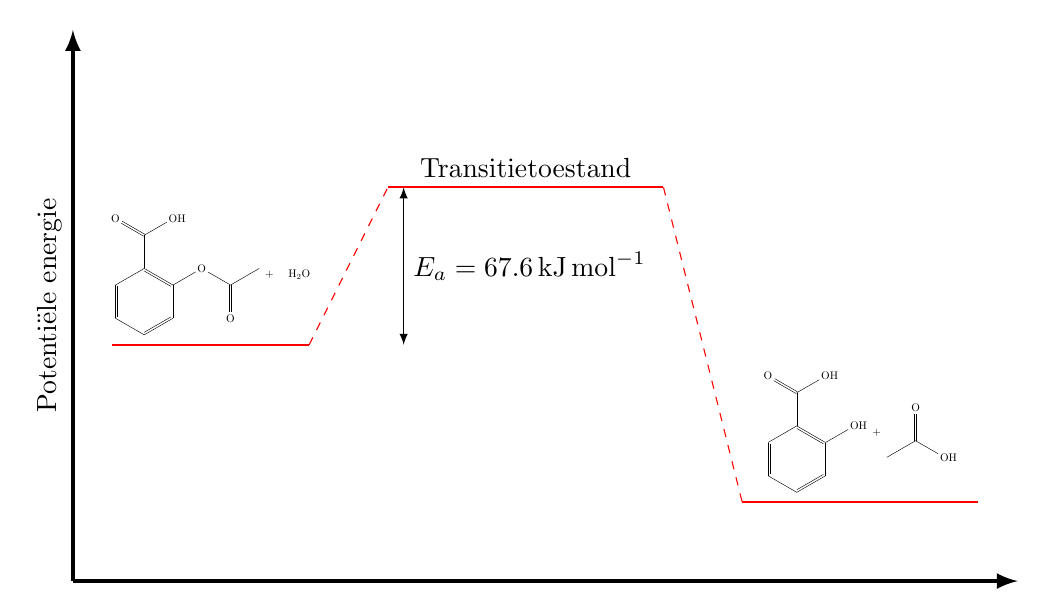
\begin{tikzpicture}
\draw[-latex,ultra thick] (0,0)--(12,0) ;
\draw[-latex,ultra thick] (0,0)--(0,7) node[midway,above,sloped]{Potenti\"ele energie};

\draw[-,thick,red] (0.5,3)--(3,3) node[midway,above,black]{\schemestart
	\scalebox{.4}{\chemfig{*6(-=-(-O-[::-60](=[::-60]O)-[::+60])=(-(=[::+60]O)-[::-60]OH)-=-)}} \arrow{0}[,0] \scalebox{.4}{\+} \scalebox{.4}{\chemfig{H_2O}}
	\schemestop};
\draw[-,red,dashed](3,3)--(4,5);
\draw[-,thick,red] (4,5)--(7.5,5)node[midway,above,black]{Transitietoestand};
\draw[-,dashed,red] (7.5,5)--(8.5,1);
\draw[-,thick,red]  (8.5,1)--(11.5,1)node[midway,above,black]{\schemestart
	\scalebox{.4}{\chemfig{*6(-=-(-OH)=(-(=[::+60]O)-[::-60]OH)-=-)}} \arrow{0}[,0] \scalebox{.4}{\+} \arrow{0}[,0]
	\scalebox{.4}{\chemfig{[:-90]O=(-[::+60]OH)-[::-60]}}
	\schemestop};

\draw[latex-latex] (4.2,3)--(4.2,5) node[midway,right,black]{$E_a = \SI{67.6}{\kilo \joule \per \mole}$}; ;


\end{tikzpicture}
\end{document}